\documentclass[times, utf8, seminar, numeric]{fer}
\usepackage{booktabs}
 \usepackage{url}

\begin{document}

% Ukljuci literaturu u seminar
\nocite{*}

\title{Poboljšanje djelomično sastavljenog genoma dugim očitanjima}

\author{Bruno Kovač, Tonko Sabolčec, Fabijan Čorak}

\voditelj{doc. dr. sc. Krešimir Križanović}

\maketitle

\tableofcontents

\chapter{Uvod}
Sekvenciranje genoma svodi se na kombiniranje očitanja u jednu cjelinu. Ovaj rad pretpostavlja da su očitanja već sastavljena, ali djelomično - u fragmente. Jedan takav fragment naziva se \textit{contig}. Dakle, zadatak se svodi na što bolje povezivanje \textit{contiga}, što smo učinili postupkom opisanim u \cite{Du345983}, koji se oslanja na duga očitanja (?). Taj rad definira nekoliko mjera preklopljenosti očitanja koje kombiniraju duljinu područja \textit{overlap} ($OL$), \textit{overhang} ($OH$) i \textit{extension} ($EL$). Mjere su ovdje definirane za dva očitanja $S_1$ i $S_2$; pripadnost područja određena je indeksom.

\begin{figure}[h]
	\centering
	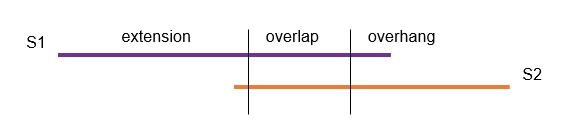
\includegraphics[width=0.7\linewidth]{img/overlap}
	\caption[]{Preklop dvaju očitanja s naznačenim područjima}
	\label{fig:overlap}
\end{figure}

\begin{itemize}
	\item \textit{sequence identity ($SI$)} - omjer ukupnog broja podudarajućih znakova u \textit{overlap} područjima i duljine duljeg od tih dvaju područja
		\[ SI = \frac{\text{broj\_podudaranja}}{\max(OL_1, OL_2)} \]
	\item \textit{overlap score ($OS$)}
		\[ OS = \left(OL_1 + OL_2\right)\frac{SI}{2} \]
	\item \textit{extension score ($ES$)} - uz $S_2$ kao produžetak od $S_1$
		\[ ES_2 = OS + \frac{EL_2 - OH_1 - OH_2}{2} \]
\end{itemize}


\chapter{Postupak}
Sastavljanje očitanja u niz modelirano je izgradnjom i obilaskom grafa.
\section{Izgradnja grafa}
Svaki \textit{contig} i svako očitanje čine jedan čvor grafa. Čvor koji predstavlja \textit{contig} zovemo \textit{anchor}. Brid postoji između svaka dva čvora čiji je $SI$ veći od nekog minimuma (u radu je uzeta vrijednost $0.97$). Pritom svaki brid nosi informacije o preklopljenosti čvorova koje povezuje ($SI$, $OS$, $ES$). Te mjere računaju se na temelju informacija o preklopljenosti dobivenih korištenjem alata \textit{minimap2} opisanog u \cite{minimap2}.

\section{Obilazak grafa}

\begin{figure}[h]
	\centering
	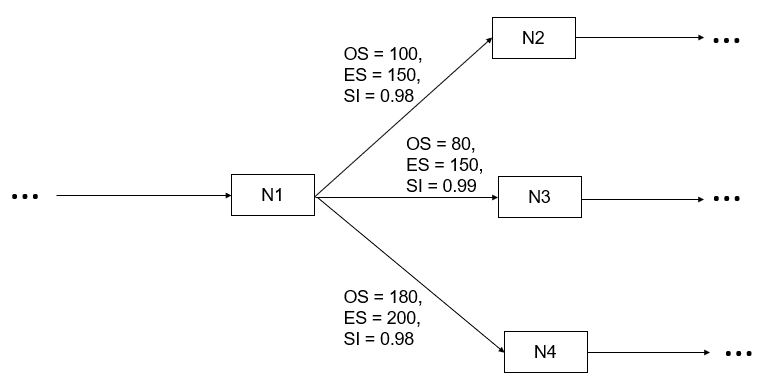
\includegraphics[width=0.7\linewidth]{img/traversal}
	\caption{Odabir sljedećeg čvora u obilasku}
	\label{fig:traversal}
\end{figure}

\noindent
Kroz graf se traže putovi čije su krajnje točke \textit{anchor} čvorovi. Za to se koriste tri načina obilaska, prilikom kojih je postavljena maksimalna dubina pretraživanja i pamte se obiđeni čvorovi:
\begin{enumerate}
	\item Iz \textit{anchor} čvora pretraga se nastavlja u sve susjedne čvorove. Iz svakog sljedećeg čvora, pretraga se nastavlja u onaj susjed s kojim je najveći \textit{overlap score}, a kojim se u konačnici dolazi do \textit{anchor} čvora. Ako je \textit{overlap score} jednak, gleda se \textit{sequence identity}. Ako je pak i ta mjera jednaka, gleda se duljina očitanja.
	\item Kao i prethodni način, ali umjesto mjere \textit{overlap score} gleda se \textit{extension score}.
	\item U svakom čvoru susjed se odabire probabilistički - s vjerojatnošću odabira proporcionalnom mjeri \textit{extension score}, sve dok se ne dosegne \textit{anchor}. Postupak se pokreće iz svakog \textit{anchor} čvora proizvoljan broj puta. Ovo je tzv. Monte Carlo metoda.
\end{enumerate}

\section{Obrada putova}
Nakon agregacije putova dobivenih trima (?) opisanim postupcima, odbacuju se duplikati i radi se odabir jednog puta za svaki par \textit{anchor} čvorova....
Conflict index?


\section{Primjer (?)}
% vizualizacijski primjer
jel dovoljno ilustrirati svaki korak, ili provođenje cijelog algoritma treba ilustrirat baš na zasebnom primjeru?

\chapter{Rezultati}
Implementacija je ispitana na uzorcima ..., ... i ... na jednoj dretvi uz procesorsku moć od ... GHz.

\begin{center}
\begin{tabular}{|c||c|c|}
	\hline
	uzorak / organizam (?) & vrijeme (s) & memorija (GiB)\\
	\hline
	\hline
	E. Coli & X & Y \\
	\hline
	A & B & C \\
	\hline
\end{tabular}
\end{center}
\chapter{Zaključak}
Zaključak.

\bibliography{literatura}
\bibliographystyle{fer}

\chapter{Sažetak}
Sažetak. ne treba nam ovo

\end{document}
